\subsection{Magnet system}

A strong magnetic field is required for precise measurement of charged particle momenta.
The ATLAS detector uses two large superconducting magnet systems, a hybrid system of a central superconducting solenoid and three outer superconducting toroids, to bend charged particles~\cite{McFayden:phdthesis}.
The total magnet system is 22 m in diameter and 26 m in length as shown in figure~\ref{fig:megnet_sys}.
\begin{figure}[!htb]
  \centering
  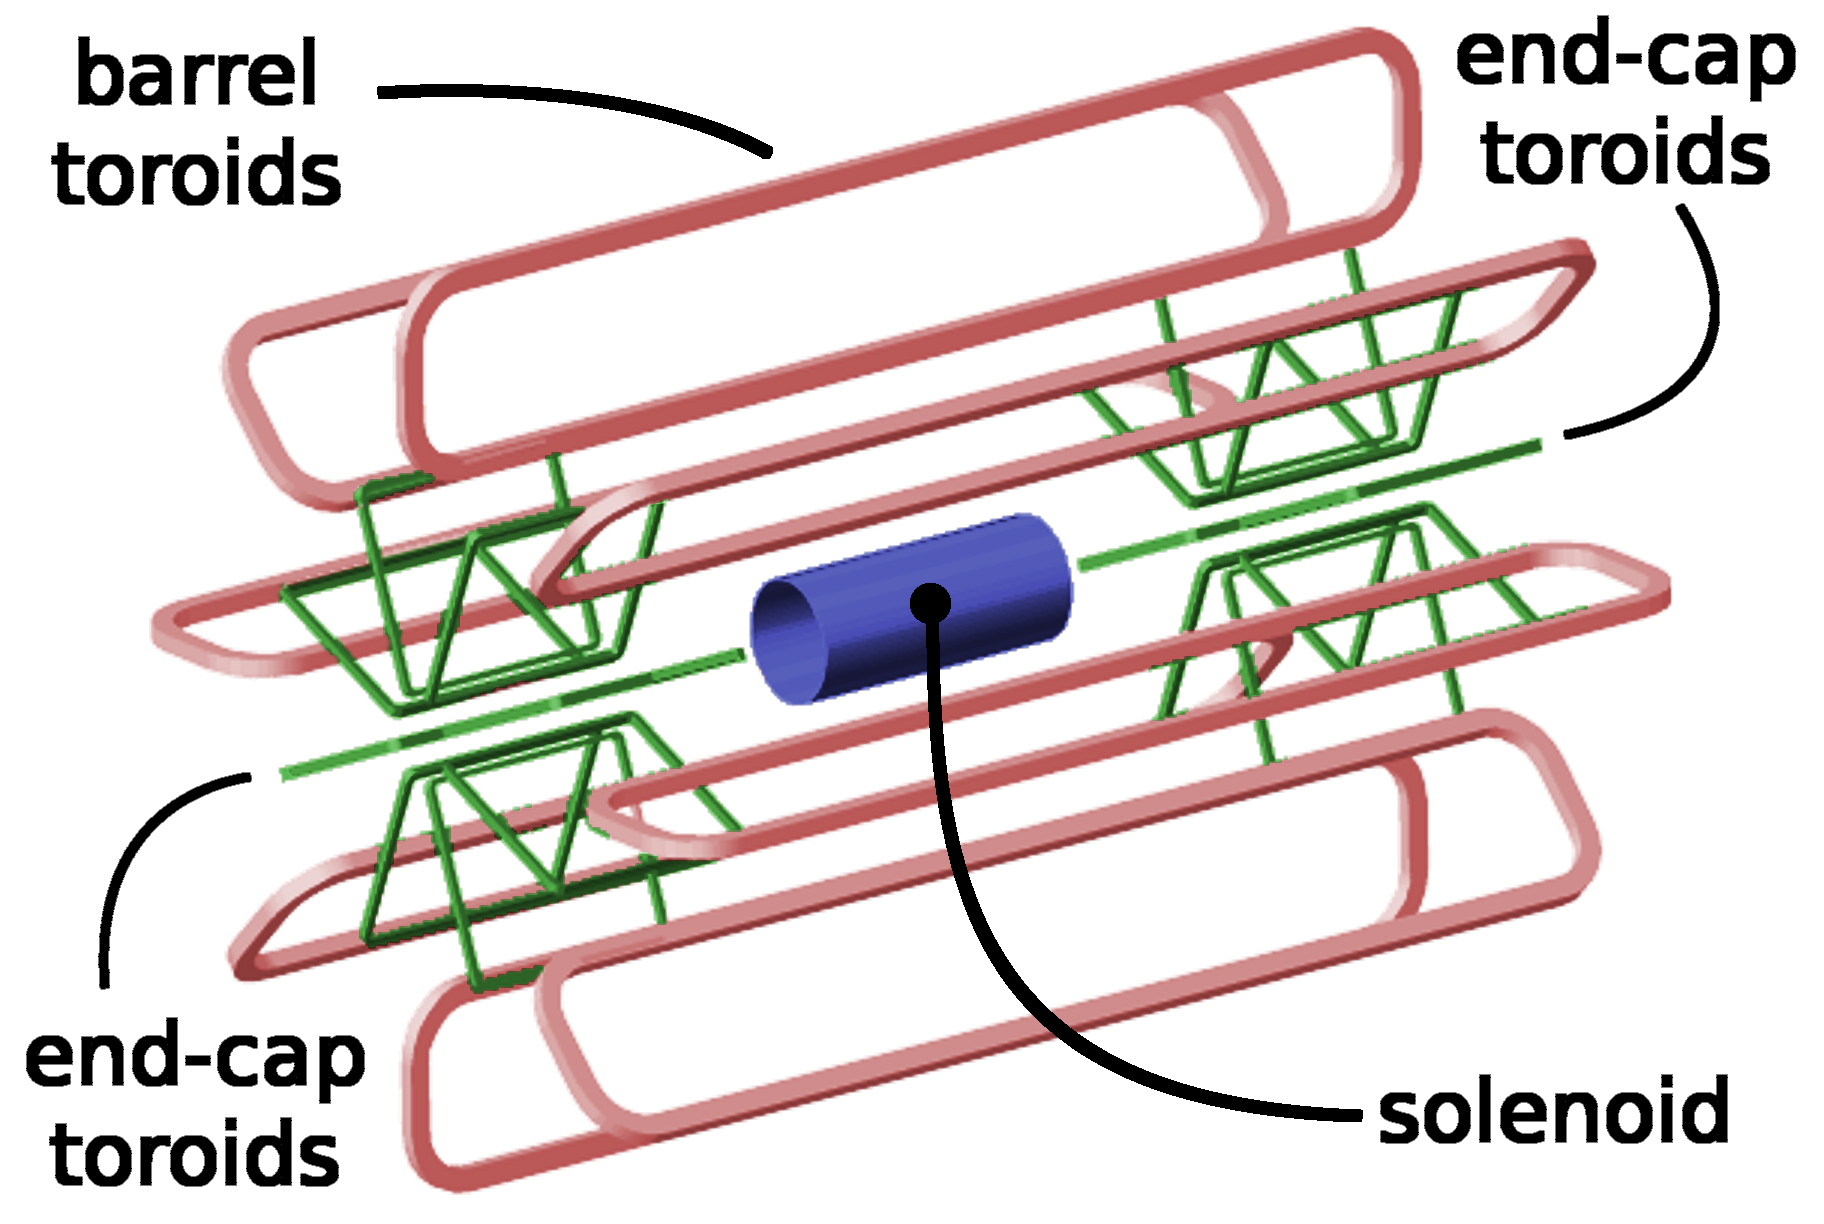
\includegraphics[width=0.7\textwidth]{figures/Detector/magnetSystems.png}
  \caption{Schematic view of the ATLAS magnet system.}
  \label{fig:megnet_sys}
\end{figure}

The central solenoid produces two Tesla magnetic field surrounding the inner Detector.
When obtaining such high field strength, at the same time, the solenoid needs to be thin in order to reduce the material in front of the calorimeter.

The outer toroid system comprises one barrel superconducting toroid and two end-caps.
The barrel one is composed of eight coils encased in individual racetrack-shaped, stainless-steel vacuum vessels and produces the magnetic field in the cylindrical volume surrounding the calorimeters.
Each end-cap toroid has one single cold mass built up from eight flat, square coil units and eight keystone wedges and provides a magnetic field of approximately 4 T for the muon detectors in the end-cap regions.
